\documentclass[twoside]{book}

% Packages required by doxygen
\usepackage{fixltx2e}
\usepackage{calc}
\usepackage{doxygen}
\usepackage[export]{adjustbox} % also loads graphicx
\usepackage{graphicx}
\usepackage[utf8]{inputenc}
\usepackage{makeidx}
\usepackage{multicol}
\usepackage{multirow}
\PassOptionsToPackage{warn}{textcomp}
\usepackage{textcomp}
\usepackage[nointegrals]{wasysym}
\usepackage[table]{xcolor}

% Font selection
\usepackage[T1]{fontenc}
\usepackage[scaled=.90]{helvet}
\usepackage{courier}
\usepackage{amssymb}
\usepackage{sectsty}
\renewcommand{\familydefault}{\sfdefault}
\allsectionsfont{%
  \fontseries{bc}\selectfont%
  \color{darkgray}%
}
\renewcommand{\DoxyLabelFont}{%
  \fontseries{bc}\selectfont%
  \color{darkgray}%
}
\newcommand{\+}{\discretionary{\mbox{\scriptsize$\hookleftarrow$}}{}{}}

% Page & text layout
\usepackage{geometry}
\geometry{%
  a4paper,%
  top=2.5cm,%
  bottom=2.5cm,%
  left=2.5cm,%
  right=2.5cm%
}
\tolerance=750
\hfuzz=15pt
\hbadness=750
\setlength{\emergencystretch}{15pt}
\setlength{\parindent}{0cm}
\setlength{\parskip}{3ex plus 2ex minus 2ex}
\makeatletter
\renewcommand{\paragraph}{%
  \@startsection{paragraph}{4}{0ex}{-1.0ex}{1.0ex}{%
    \normalfont\normalsize\bfseries\SS@parafont%
  }%
}
\renewcommand{\subparagraph}{%
  \@startsection{subparagraph}{5}{0ex}{-1.0ex}{1.0ex}{%
    \normalfont\normalsize\bfseries\SS@subparafont%
  }%
}
\makeatother

% Headers & footers
\usepackage{fancyhdr}
\pagestyle{fancyplain}
\fancyhead[LE]{\fancyplain{}{\bfseries\thepage}}
\fancyhead[CE]{\fancyplain{}{}}
\fancyhead[RE]{\fancyplain{}{\bfseries\leftmark}}
\fancyhead[LO]{\fancyplain{}{\bfseries\rightmark}}
\fancyhead[CO]{\fancyplain{}{}}
\fancyhead[RO]{\fancyplain{}{\bfseries\thepage}}
\fancyfoot[LE]{\fancyplain{}{}}
\fancyfoot[CE]{\fancyplain{}{}}
\fancyfoot[RE]{\fancyplain{}{\bfseries\scriptsize Generated by Doxygen }}
\fancyfoot[LO]{\fancyplain{}{\bfseries\scriptsize Generated by Doxygen }}
\fancyfoot[CO]{\fancyplain{}{}}
\fancyfoot[RO]{\fancyplain{}{}}
\renewcommand{\footrulewidth}{0.4pt}
\renewcommand{\chaptermark}[1]{%
  \markboth{#1}{}%
}
\renewcommand{\sectionmark}[1]{%
  \markright{\thesection\ #1}%
}

% Indices & bibliography
\usepackage{natbib}
\usepackage[titles]{tocloft}
\setcounter{tocdepth}{3}
\setcounter{secnumdepth}{5}
\makeindex

% Hyperlinks (required, but should be loaded last)
\usepackage{ifpdf}
\ifpdf
  \usepackage[pdftex,pagebackref=true]{hyperref}
\else
  \usepackage[ps2pdf,pagebackref=true]{hyperref}
\fi
\hypersetup{%
  colorlinks=true,%
  linkcolor=blue,%
  citecolor=blue,%
  unicode%
}

% Custom commands
\newcommand{\clearemptydoublepage}{%
  \newpage{\pagestyle{empty}\cleardoublepage}%
}

\usepackage{caption}
\captionsetup{labelsep=space,justification=centering,font={bf},singlelinecheck=off,skip=4pt,position=top}

%===== C O N T E N T S =====

\begin{document}

% Titlepage & ToC
\hypersetup{pageanchor=false,
             bookmarksnumbered=true,
             pdfencoding=unicode
            }
\pagenumbering{alph}
\begin{titlepage}
\vspace*{7cm}
\begin{center}%
{\Large Hexapod\+\_\+\+Team\+Project }\\
\vspace*{1cm}
{\large Generated by Doxygen 1.8.14}\\
\end{center}
\end{titlepage}
\clearemptydoublepage
\pagenumbering{roman}
\tableofcontents
\clearemptydoublepage
\pagenumbering{arabic}
\hypersetup{pageanchor=true}

%--- Begin generated contents ---
\chapter{Hierarchical Index}
\section{Class Hierarchy}
This inheritance list is sorted roughly, but not completely, alphabetically\+:\begin{DoxyCompactList}
\item \contentsline{section}{Bluetooth\+Interface}{\pageref{class_bluetooth_interface}}{}
\item \contentsline{section}{Leg}{\pageref{class_leg}}{}
\item \contentsline{section}{Motion\+Sequence}{\pageref{class_motion_sequence}}{}
\begin{DoxyCompactList}
\item \contentsline{section}{Pt\+P\+Motion}{\pageref{class_pt_p_motion}}{}
\end{DoxyCompactList}
\item \contentsline{section}{Movement\+Controller}{\pageref{class_movement_controller}}{}
\item \contentsline{section}{Robot\+Control}{\pageref{class_robot_control}}{}
\item \contentsline{section}{Servo}{\pageref{class_servo}}{}
\end{DoxyCompactList}

\chapter{Class Index}
\section{Class List}
Here are the classes, structs, unions and interfaces with brief descriptions\+:\begin{DoxyCompactList}
\item\contentsline{section}{\mbox{\hyperlink{class_bluetooth_interface}{Bluetooth\+Interface}} }{\pageref{class_bluetooth_interface}}{}
\item\contentsline{section}{\mbox{\hyperlink{class_leg}{Leg}} }{\pageref{class_leg}}{}
\item\contentsline{section}{\mbox{\hyperlink{class_motion_sequence}{Motion\+Sequence}} }{\pageref{class_motion_sequence}}{}
\item\contentsline{section}{\mbox{\hyperlink{class_movement_controller}{Movement\+Controller}} }{\pageref{class_movement_controller}}{}
\item\contentsline{section}{\mbox{\hyperlink{class_pt_p_motion}{Pt\+P\+Motion}} }{\pageref{class_pt_p_motion}}{}
\item\contentsline{section}{\mbox{\hyperlink{class_robot_control}{Robot\+Control}} }{\pageref{class_robot_control}}{}
\item\contentsline{section}{\mbox{\hyperlink{class_servo}{Servo}} }{\pageref{class_servo}}{}
\end{DoxyCompactList}

\chapter{File Index}
\section{File List}
Here is a list of all documented files with brief descriptions\+:\begin{DoxyCompactList}
\item\contentsline{section}{{\bfseries Bluetooth\+Interface.\+h} }{\pageref{_bluetooth_interface_8h}}{}
\item\contentsline{section}{{\bfseries Leg.\+h} }{\pageref{_leg_8h}}{}
\item\contentsline{section}{{\bfseries Motion\+Sequence.\+h} }{\pageref{_motion_sequence_8h}}{}
\item\contentsline{section}{\mbox{\hyperlink{_movement_controller_8cpp}{Movement\+Controller.\+cpp}} }{\pageref{_movement_controller_8cpp}}{}
\item\contentsline{section}{\mbox{\hyperlink{_movement_controller_8h}{Movement\+Controller.\+h}} }{\pageref{_movement_controller_8h}}{}
\item\contentsline{section}{{\bfseries Pt\+P\+Motion.\+h} }{\pageref{_pt_p_motion_8h}}{}
\item\contentsline{section}{{\bfseries Robot\+Control.\+h} }{\pageref{_robot_control_8h}}{}
\item\contentsline{section}{{\bfseries Servo.\+h} }{\pageref{_servo_8h}}{}
\item\contentsline{section}{\+\_\+\+\_\+vm/{\bfseries .\+Hexapod\+\_\+\+Team\+Project.\+vsarduino.\+h} }{\pageref{_8_hexapod___team_project_8vsarduino_8h}}{}
\end{DoxyCompactList}

\chapter{Class Documentation}
\hypertarget{class_bluetooth_interface}{}\section{Bluetooth\+Interface Class Reference}
\label{class_bluetooth_interface}\index{Bluetooth\+Interface@{Bluetooth\+Interface}}
\subsection*{Public Member Functions}
\begin{DoxyCompactItemize}
\item 
\mbox{\Hypertarget{class_bluetooth_interface_a4ae2135ffda7217b3ee6b2c446eed6db}\label{class_bluetooth_interface_a4ae2135ffda7217b3ee6b2c446eed6db}} 
unsigned char {\bfseries read\+Input} ()
\item 
\mbox{\Hypertarget{class_bluetooth_interface_a54f6e0ae1122c5efc2f08873b4ec1100}\label{class_bluetooth_interface_a54f6e0ae1122c5efc2f08873b4ec1100}} 
int {\bfseries get\+DirectionX} ()
\item 
\mbox{\Hypertarget{class_bluetooth_interface_aeb5f167f9ea6e4c114ebe8a608d40ba0}\label{class_bluetooth_interface_aeb5f167f9ea6e4c114ebe8a608d40ba0}} 
int {\bfseries get\+DirectionY} ()
\item 
\mbox{\Hypertarget{class_bluetooth_interface_a0c6f6b97c385a336187de2b02a08e754}\label{class_bluetooth_interface_a0c6f6b97c385a336187de2b02a08e754}} 
int {\bfseries get\+DirectionZ} ()
\item 
\mbox{\Hypertarget{class_bluetooth_interface_a547308ab89e836ccb290ac821b538320}\label{class_bluetooth_interface_a547308ab89e836ccb290ac821b538320}} 
int {\bfseries calc\+Angle} (int app\+Value)
\end{DoxyCompactItemize}
\subsection*{Public Attributes}
\begin{DoxyCompactItemize}
\item 
\mbox{\Hypertarget{class_bluetooth_interface_aa8abc129f546e58e0cd8f9e88db61802}\label{class_bluetooth_interface_aa8abc129f546e58e0cd8f9e88db61802}} 
char {\bfseries app\+Value}
\item 
\mbox{\Hypertarget{class_bluetooth_interface_ac97f1946092309df55a13162e095e964}\label{class_bluetooth_interface_ac97f1946092309df55a13162e095e964}} 
int {\bfseries m\+\_\+diretionX}
\item 
\mbox{\Hypertarget{class_bluetooth_interface_a70250fa08d5535491e24bf629aa8dc5a}\label{class_bluetooth_interface_a70250fa08d5535491e24bf629aa8dc5a}} 
int {\bfseries m\+\_\+diretionY}
\item 
\mbox{\Hypertarget{class_bluetooth_interface_ab5c2891fdaaa0a292ce20d8e58fd4ea2}\label{class_bluetooth_interface_ab5c2891fdaaa0a292ce20d8e58fd4ea2}} 
int {\bfseries m\+\_\+diretionZ}
\end{DoxyCompactItemize}


The documentation for this class was generated from the following files\+:\begin{DoxyCompactItemize}
\item 
Bluetooth\+Interface.\+h\item 
Bluetooth\+Interface.\+cpp\end{DoxyCompactItemize}

\hypertarget{class_leg}{}\section{Leg Class Reference}
\label{class_leg}\index{Leg@{Leg}}
\subsection*{Public Member Functions}
\begin{DoxyCompactItemize}
\item 
\mbox{\Hypertarget{class_leg_ab3490019b9bbb3a8bcc32691bf5a6e75}\label{class_leg_ab3490019b9bbb3a8bcc32691bf5a6e75}} 
{\bfseries Leg} (A\+X12A \&m\+\_\+p\+Connected\+Bus, unsigned char I\+D\+\_\+body\+Servo, unsigned char I\+D\+\_\+middle\+Leg\+Servo, unsigned char I\+D\+\_\+lower\+Leg\+Servo)
\item 
\mbox{\Hypertarget{class_leg_a62128cac5af3c307cb7a836d660c4a93}\label{class_leg_a62128cac5af3c307cb7a836d660c4a93}} 
unsigned char {\bfseries move2\+Home\+Position} ()
\item 
\mbox{\Hypertarget{class_leg_a7e1d28688ebca828c02eb69d29440701}\label{class_leg_a7e1d28688ebca828c02eb69d29440701}} 
unsigned char {\bfseries lift\+Leg} ()
\item 
\mbox{\Hypertarget{class_leg_a4c42b41dc29e07e35a82856addb9e2c7}\label{class_leg_a4c42b41dc29e07e35a82856addb9e2c7}} 
unsigned char {\bfseries drop\+Leg} ()
\item 
\mbox{\Hypertarget{class_leg_ad65204bbf94601d091e775b011bc0ac4}\label{class_leg_ad65204bbf94601d091e775b011bc0ac4}} 
unsigned char {\bfseries move\+Leg\+To\+Known\+Position} (float angle\+Body, float angle\+Middle, float angle\+Lower, float pk\+Xnew, float pk\+Ynew, float pk\+Znew)
\item 
\mbox{\Hypertarget{class_leg_a1cabc989ff35134313cff1c6349fa5ed}\label{class_leg_a1cabc989ff35134313cff1c6349fa5ed}} 
unsigned char {\bfseries set\+Body\+Servo\+Angle} (float angle)
\item 
\mbox{\Hypertarget{class_leg_a66cf5a6988aa5533dd22999de75494d5}\label{class_leg_a66cf5a6988aa5533dd22999de75494d5}} 
unsigned char {\bfseries set\+Middle\+Servo\+Angle} (float angle)
\item 
\mbox{\Hypertarget{class_leg_a996c44acd7afbdaa955614535492ff2b}\label{class_leg_a996c44acd7afbdaa955614535492ff2b}} 
unsigned char {\bfseries set\+Lower\+Servo\+Angle} (float angle)
\end{DoxyCompactItemize}
\subsection*{Public Attributes}
\begin{DoxyCompactItemize}
\item 
\mbox{\Hypertarget{class_leg_ad524af2808920c519a12fbf39dd3b085}\label{class_leg_ad524af2808920c519a12fbf39dd3b085}} 
A\+X12A $\ast$ {\bfseries m\+\_\+p\+Connected\+Bus}
\item 
\mbox{\Hypertarget{class_leg_a2e216786fe3fd6a86abc6dd64b94e355}\label{class_leg_a2e216786fe3fd6a86abc6dd64b94e355}} 
\mbox{\hyperlink{class_servo}{Servo}} {\bfseries m\+\_\+body\+Servo}
\item 
\mbox{\Hypertarget{class_leg_a76504a55bf5fa10ca4c017f4d8e40a31}\label{class_leg_a76504a55bf5fa10ca4c017f4d8e40a31}} 
\mbox{\hyperlink{class_servo}{Servo}} {\bfseries m\+\_\+middle\+Servo}
\item 
\mbox{\Hypertarget{class_leg_a8c384fd114b68f4e9ee1eded87d0bf8b}\label{class_leg_a8c384fd114b68f4e9ee1eded87d0bf8b}} 
\mbox{\hyperlink{class_servo}{Servo}} {\bfseries m\+\_\+lower\+Servo}
\end{DoxyCompactItemize}


The documentation for this class was generated from the following files\+:\begin{DoxyCompactItemize}
\item 
Leg.\+h\item 
Leg.\+cpp\end{DoxyCompactItemize}

\hypertarget{class_motion_sequence}{}\section{Motion\+Sequence Class Reference}
\label{class_motion_sequence}\index{Motion\+Sequence@{Motion\+Sequence}}
Inheritance diagram for Motion\+Sequence\+:\begin{figure}[H]
\begin{center}
\leavevmode
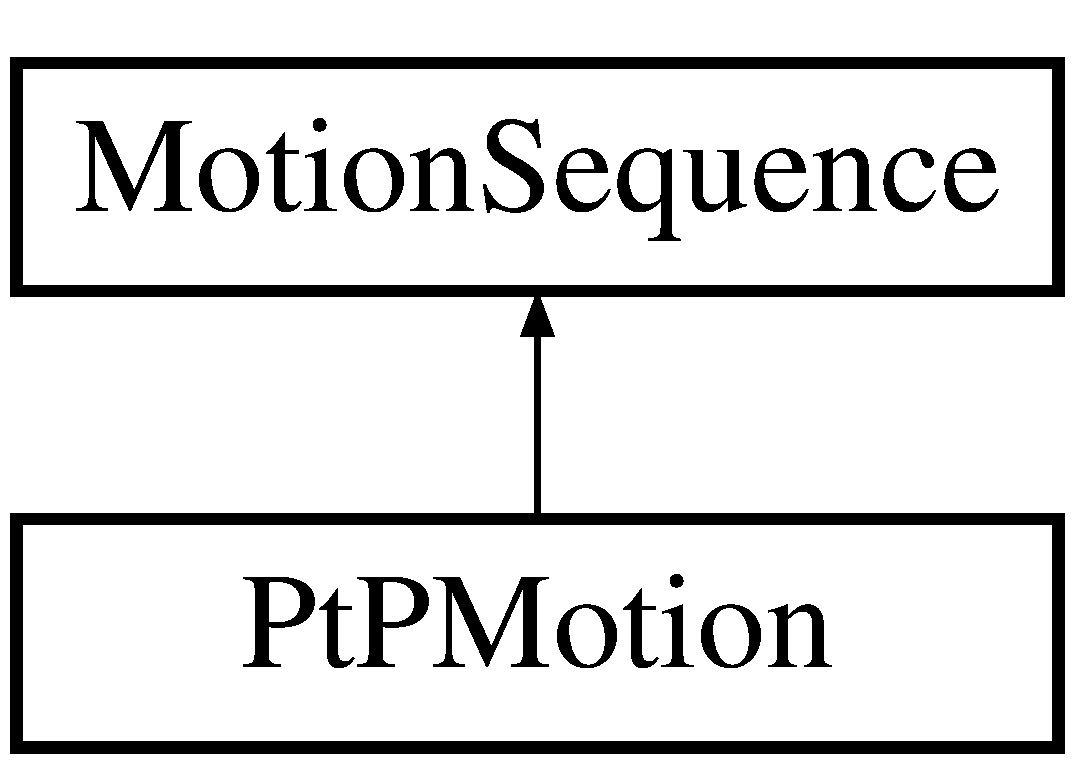
\includegraphics[height=2.000000cm]{class_motion_sequence}
\end{center}
\end{figure}
\subsection*{Public Member Functions}
\begin{DoxyCompactItemize}
\item 
\mbox{\Hypertarget{class_motion_sequence_aeccbbc93c854052e3b0ba01cebee6633}\label{class_motion_sequence_aeccbbc93c854052e3b0ba01cebee6633}} 
{\bfseries Motion\+Sequence} (int size, Speed\+Mode val\+Speed\+Mode, Position\+Mode val\+Position\+Mode)
\item 
\mbox{\Hypertarget{class_motion_sequence_ac0325367b2704b0d2f845f8069ef4b0a}\label{class_motion_sequence_ac0325367b2704b0d2f845f8069ef4b0a}} 
int {\bfseries get\+Size} ()
\item 
\mbox{\Hypertarget{class_motion_sequence_a68166f9582eae38f2aa137a869443387}\label{class_motion_sequence_a68166f9582eae38f2aa137a869443387}} 
unsigned char {\bfseries get\+Angle\+Sequence\+At} (int index, float \&val\+Q1, float \&val\+Q2, float \&val\+Q3)
\item 
\mbox{\Hypertarget{class_motion_sequence_a455d0103a3df19a1a0ea14cbe9a5facc}\label{class_motion_sequence_a455d0103a3df19a1a0ea14cbe9a5facc}} 
unsigned char {\bfseries get\+Velocity\+Sequence\+At} (int index, float \&val\+V\+Q1, float \&val\+V\+Q2, float \&val\+V\+Q3)
\item 
\mbox{\Hypertarget{class_motion_sequence_a5f6349cb0b1e5916acfd9a9a165519b6}\label{class_motion_sequence_a5f6349cb0b1e5916acfd9a9a165519b6}} 
unsigned char {\bfseries get\+Motion\+Sequence\+At} (int index, float \&valX, float \&valY, float \&valZ)
\item 
\mbox{\Hypertarget{class_motion_sequence_a8865eb9528ee86c93d9f2d2be58dd55b}\label{class_motion_sequence_a8865eb9528ee86c93d9f2d2be58dd55b}} 
float {\bfseries get\+Q1\+Angle\+Sequence\+At} (int index)
\item 
\mbox{\Hypertarget{class_motion_sequence_a9be53be839ed033b0d551dcf74c6a8a2}\label{class_motion_sequence_a9be53be839ed033b0d551dcf74c6a8a2}} 
float {\bfseries get\+Q2\+Angle\+Sequence\+At} (int index)
\item 
\mbox{\Hypertarget{class_motion_sequence_aa7bb8a17554cda64c2e5dbd6af1d25cb}\label{class_motion_sequence_aa7bb8a17554cda64c2e5dbd6af1d25cb}} 
float {\bfseries get\+Q3\+Angle\+Sequence\+At} (int index)
\item 
\mbox{\Hypertarget{class_motion_sequence_a4a03996f66ded7ea006a9de3af99fdad}\label{class_motion_sequence_a4a03996f66ded7ea006a9de3af99fdad}} 
float {\bfseries get\+X\+Motion\+Sequence\+At} (int index)
\item 
\mbox{\Hypertarget{class_motion_sequence_a729ff79656c2ab6e4e9a2e60459d98da}\label{class_motion_sequence_a729ff79656c2ab6e4e9a2e60459d98da}} 
float {\bfseries get\+Y\+Motion\+Sequence\+At} (int index)
\item 
\mbox{\Hypertarget{class_motion_sequence_a3311b61763e3718f6ed132a43d55d846}\label{class_motion_sequence_a3311b61763e3718f6ed132a43d55d846}} 
float {\bfseries get\+Z\+Motion\+Sequence\+At} (int index)
\item 
\mbox{\Hypertarget{class_motion_sequence_a27ff1becf72db7e18cede87ae531c612}\label{class_motion_sequence_a27ff1becf72db7e18cede87ae531c612}} 
unsigned char {\bfseries set\+Angle\+Sequence\+At} (int index, float val\+Q1, float val\+Q2, float val\+Q3)
\item 
\mbox{\Hypertarget{class_motion_sequence_a682065eef7969f3029ba6c813096f32c}\label{class_motion_sequence_a682065eef7969f3029ba6c813096f32c}} 
unsigned char {\bfseries set\+Velocity\+Sequence\+At} (int index, float val\+V\+Q1, float val\+V\+Q2, float val\+V\+Q3)
\item 
\mbox{\Hypertarget{class_motion_sequence_adff7296e0da1e39a1986fae306a647f9}\label{class_motion_sequence_adff7296e0da1e39a1986fae306a647f9}} 
unsigned char {\bfseries set\+Motion\+Sequence\+At} (int index, float valX, float valY, float valZ)
\end{DoxyCompactItemize}


The documentation for this class was generated from the following files\+:\begin{DoxyCompactItemize}
\item 
Motion\+Sequence.\+h\item 
Motion\+Sequence.\+cpp\end{DoxyCompactItemize}

\hypertarget{class_movement_controller}{}\section{Movement\+Controller Class Reference}
\label{class_movement_controller}\index{Movement\+Controller@{Movement\+Controller}}


{\ttfamily \#include $<$Movement\+Controller.\+h$>$}

\subsection*{Public Member Functions}
\begin{DoxyCompactItemize}
\item 
\mbox{\Hypertarget{class_movement_controller_aed25a9c08f44c223108137bc932ddd35}\label{class_movement_controller_aed25a9c08f44c223108137bc932ddd35}} 
unsigned char {\bfseries init\+Robot} ()
\item 
\mbox{\Hypertarget{class_movement_controller_a2c60a9e0f4750a9ffa08196270795166}\label{class_movement_controller_a2c60a9e0f4750a9ffa08196270795166}} 
unsigned char {\bfseries move2\+Home\+Position} ()
\end{DoxyCompactItemize}
\begin{Indent}\textbf{ world\+Coordinates\+To\+Leg\+Coordinates}\par
{\em Converts world coordinates to the specific leg coordinate system. }\begin{DoxyCompactItemize}
\item 
unsigned char \mbox{\hyperlink{class_movement_controller_a0710b423644d46f7391e4b75c5879559}{get\+Leg\+Coordinates\+From\+World\+Coordinates}} (unsigned char leg\+Number, float pk\+Xold, float pk\+Yold, float pk\+Zold, float pwX, float pwY, float pwZ, float \&pkX, float \&pkY, float \&pkZ)
\item 
\mbox{\Hypertarget{class_movement_controller_a328939445cf5c8f7878e9fd44fde3c96}\label{class_movement_controller_a328939445cf5c8f7878e9fd44fde3c96}} 
unsigned char {\bfseries world\+Position\+To\+Leg\+One\+Position} (float pk\+Xold, float pk\+Yold, float pk\+Zold, float pwX, float pwY, float pwZ, float \&pkX, float \&pkY, float \&pkZ)
\item 
\mbox{\Hypertarget{class_movement_controller_a715ebda5d6d77f1763d0288268caf5ae}\label{class_movement_controller_a715ebda5d6d77f1763d0288268caf5ae}} 
unsigned char {\bfseries world\+Position\+To\+Leg\+Two\+Position} (float pk\+Xold, float pk\+Yold, float pk\+Zold, float pwX, float pwY, float pwZ, float \&pkX, float \&pkY, float \&pkZ)
\item 
\mbox{\Hypertarget{class_movement_controller_a1c4c708534a712257c7282638568e9ee}\label{class_movement_controller_a1c4c708534a712257c7282638568e9ee}} 
unsigned char {\bfseries world\+Position\+To\+Leg\+Three\+Position} (float pk\+Xold, float pk\+Yold, float pk\+Zold, float pwX, float pwY, float pwZ, float \&pkX, float \&pkY, float \&pkZ)
\item 
\mbox{\Hypertarget{class_movement_controller_a5ebb5b6f2242350310aede085140cffe}\label{class_movement_controller_a5ebb5b6f2242350310aede085140cffe}} 
unsigned char {\bfseries world\+Position\+To\+Leg\+Four\+Position} (float pk\+Xold, float pk\+Yold, float pk\+Zold, float pwX, float pwY, float pwZ, float \&pkX, float \&pkY, float \&pkZ)
\item 
\mbox{\Hypertarget{class_movement_controller_ad57ba364952a497b5772c67cc27ed797}\label{class_movement_controller_ad57ba364952a497b5772c67cc27ed797}} 
unsigned char {\bfseries world\+Position\+To\+Leg\+Five\+Position} (float pk\+Xold, float pk\+Yold, float pk\+Zold, float pwX, float pwY, float pwZ, float \&pkX, float \&pkY, float \&pkZ)
\item 
\mbox{\Hypertarget{class_movement_controller_ac8928ae991954ef78fc32c9faa0d0c54}\label{class_movement_controller_ac8928ae991954ef78fc32c9faa0d0c54}} 
unsigned char {\bfseries world\+Position\+To\+Leg\+Six\+Position} (float pk\+Xold, float pk\+Yold, float pk\+Zold, float pwX, float pwY, float pwZ, float \&pkX, float \&pkY, float \&pkZ)
\end{DoxyCompactItemize}
\end{Indent}
\begin{Indent}\textbf{ get\+World\+Coordinates\+From\+FK}\par
\begin{DoxyCompactItemize}
\item 
\mbox{\Hypertarget{class_movement_controller_a252a8052b283372152f3376ea0aee55b}\label{class_movement_controller_a252a8052b283372152f3376ea0aee55b}} 
unsigned char {\bfseries get\+World\+Coordinates\+From\+FK} (unsigned char leg\+Number, float q1, float q2, float q3, float \&px, float \&py, float \&pz)
\item 
\mbox{\Hypertarget{class_movement_controller_a3c86e9f08423c5662e2134736160d539}\label{class_movement_controller_a3c86e9f08423c5662e2134736160d539}} 
unsigned char {\bfseries leg\+One\+F\+K\+Calculation} (float q1, float q2, float q3, float \&px, float \&py, float \&pz)
\item 
\mbox{\Hypertarget{class_movement_controller_ad1349ca3157f098be97571752e55d734}\label{class_movement_controller_ad1349ca3157f098be97571752e55d734}} 
unsigned char {\bfseries leg\+Two\+F\+K\+Calculation} (float q1, float q2, float q3, float \&px, float \&py, float \&pz)
\item 
\mbox{\Hypertarget{class_movement_controller_a30eeaacb6e169c727c4892c65fd2580f}\label{class_movement_controller_a30eeaacb6e169c727c4892c65fd2580f}} 
unsigned char {\bfseries leg\+Three\+F\+K\+Calculation} (float q1, float q2, float q3, float \&px, float \&py, float \&pz)
\item 
\mbox{\Hypertarget{class_movement_controller_ab5811a162191979ea4815219fa9709e9}\label{class_movement_controller_ab5811a162191979ea4815219fa9709e9}} 
unsigned char {\bfseries leg\+Four\+F\+K\+Calculation} (float q1, float q2, float q3, float \&px, float \&py, float \&pz)
\item 
\mbox{\Hypertarget{class_movement_controller_aa1c69d5fe2c7e17ba23de283f85c38a2}\label{class_movement_controller_aa1c69d5fe2c7e17ba23de283f85c38a2}} 
unsigned char {\bfseries leg\+Five\+F\+K\+Calculation} (float q1, float q2, float q3, float \&px, float \&py, float \&pz)
\item 
\mbox{\Hypertarget{class_movement_controller_ab342cee1b0fec3faed3e98c23f50d941}\label{class_movement_controller_ab342cee1b0fec3faed3e98c23f50d941}} 
unsigned char {\bfseries leg\+Six\+F\+K\+Calculation} (float q1, float q2, float q3, float \&px, float \&py, float \&pz)
\item 
unsigned char \mbox{\hyperlink{class_movement_controller_a5765726eb4e820a7ac669c88fe4937e7}{get\+Angle\+With\+I\+K\+\_\+tan\+Formula}} (float px, float py, float pz, float \&q1, float \&q2, float \&q3)
\item 
unsigned char \mbox{\hyperlink{class_movement_controller_a53b401947106872656c4fb1e77b04bba}{interpolation\+Angle\+Endposition}} (float qend, float qhome, float(\&interpolated\+Angle\+Movement)\mbox{[}10\mbox{]}, float \&movement\+Speed)
\item 
\mbox{\Hypertarget{class_movement_controller_a12ad030f9459004052685722bc56acfb}\label{class_movement_controller_a12ad030f9459004052685722bc56acfb}} 
unsigned char {\bfseries interpolation\+Angle\+For\+Sync\+Lin\+Movement} (float deltaQ, float tb, float tv, float $\ast$interpolated\+Angle\+Movement, float $\ast$interpolated\+Velocity, int size)
\item 
\mbox{\Hypertarget{class_movement_controller_ae58ec5af97b9f1c65c375a779c77cd16}\label{class_movement_controller_ae58ec5af97b9f1c65c375a779c77cd16}} 
unsigned char {\bfseries move\+Leg\+One\+With\+Interpolated\+Position} (float q1old, float q2old, float q3old, float q1, float q2, float q3)
\item 
unsigned char \mbox{\hyperlink{class_movement_controller_a53d19d2516a2ed440c2b15fc47ea91b7}{get\+Angle\+With\+IK}} (float px, float py, float pz, float \&q1, float \&q2, float \&q3)
\item 
\mbox{\Hypertarget{class_movement_controller_a60394fc92c5874689cb4108f0d67a66a}\label{class_movement_controller_a60394fc92c5874689cb4108f0d67a66a}} 
unsigned char {\bfseries move\+Legs} (float pxold, float pyold, float pzold, float px, float py, float pz)
\item 
\mbox{\Hypertarget{class_movement_controller_a0d83341f49565d8ddf9f08e80ffed7a3}\label{class_movement_controller_a0d83341f49565d8ddf9f08e80ffed7a3}} 
unsigned char {\bfseries do\+One\+Step} (float px, float py, float pz)
\item 
\mbox{\Hypertarget{class_movement_controller_a820b51c9a23a4a363274bc28c5393295}\label{class_movement_controller_a820b51c9a23a4a363274bc28c5393295}} 
{\bfseries $\sim$\+Movement\+Controller} ()
\end{DoxyCompactItemize}
\end{Indent}
\subsection*{Public Attributes}
\textbf{ }\par
\begin{DoxyCompactItemize}
\item 
A\+X12A \mbox{\hyperlink{class_movement_controller_ac4642ac20e0affff60ff0b8c0e5efdbb}{m\+\_\+\+Servo\+Com\+Object1}}
\begin{DoxyCompactList}\small\item\em Three objects of the class A\+X12A are created. To enable parallel communication with three serial ports on the Arduino. \end{DoxyCompactList}\item 
A\+X12A \mbox{\hyperlink{class_movement_controller_abd74aff807ff311c6891311414ae3993}{m\+\_\+\+Servo\+Com\+Object2}}
\item 
A\+X12A \mbox{\hyperlink{class_movement_controller_afbe7c5a0e099b5e879d64b6ab72f7127}{m\+\_\+\+Servo\+Com\+Object3}}
\end{DoxyCompactItemize}

\textbf{ }\par
\begin{DoxyCompactItemize}
\item 
\mbox{\Hypertarget{class_movement_controller_a13bd6406481979df9aa10857a38d3381}\label{class_movement_controller_a13bd6406481979df9aa10857a38d3381}} 
\mbox{\hyperlink{class_leg}{Leg}} \mbox{\hyperlink{class_movement_controller_a13bd6406481979df9aa10857a38d3381}{m\+\_\+\+Leg1}}
\begin{DoxyCompactList}\small\item\em Every leg on the hexapod can be individually controlled by following objects. \end{DoxyCompactList}\item 
\mbox{\Hypertarget{class_movement_controller_a98baf7599b6b5c5a4dc852301dc19268}\label{class_movement_controller_a98baf7599b6b5c5a4dc852301dc19268}} 
\mbox{\hyperlink{class_leg}{Leg}} {\bfseries m\+\_\+\+Leg2}
\item 
\mbox{\Hypertarget{class_movement_controller_a0d4edfeb6b4c2ad57dd3b1e387bc4de9}\label{class_movement_controller_a0d4edfeb6b4c2ad57dd3b1e387bc4de9}} 
\mbox{\hyperlink{class_leg}{Leg}} {\bfseries m\+\_\+\+Leg3}
\item 
\mbox{\Hypertarget{class_movement_controller_a8f776e74969ff7983f6cc6909e1dec27}\label{class_movement_controller_a8f776e74969ff7983f6cc6909e1dec27}} 
\mbox{\hyperlink{class_leg}{Leg}} {\bfseries m\+\_\+\+Leg4}
\item 
\mbox{\Hypertarget{class_movement_controller_aa72587ce1fb41820aa9a8f3b94496e69}\label{class_movement_controller_aa72587ce1fb41820aa9a8f3b94496e69}} 
\mbox{\hyperlink{class_leg}{Leg}} {\bfseries m\+\_\+\+Leg5}
\item 
\mbox{\Hypertarget{class_movement_controller_a7844bc42dba768e27bb5eb86bea99ef6}\label{class_movement_controller_a7844bc42dba768e27bb5eb86bea99ef6}} 
\mbox{\hyperlink{class_leg}{Leg}} {\bfseries m\+\_\+\+Leg6}
\end{DoxyCompactItemize}



\subsection{Detailed Description}
Rough structure of the hexapod to understand the naming of the six legs. To find the \char`\"{}\+U\+P\char`\"{} position please look on the backside of the robot. 
\begin{DoxyPre}
\begin{DoxyVerb}leg1                  leg2
<===\     /"UP"\     /===>
     \==|--------|==/
        |--------|
leg3    |--------|  leg4
<=======|--------|=======>
        |--------|
        |--------|
leg5 /==|--------|==\leg6
<===/   |--------|   \===>
\end{DoxyVerb}

\end{DoxyPre}
 ~\newline
Rough structure of the hexapod to understand the naming of the three servos on one leg. \begin{DoxyVerb}         (LeftLeg)                      Hexapod                          (RightLeg) 
                            /////######################\\\\\        
       _____________     BodyServo                   BodyServo          _____________
       LowerLegServo      /////#########################\\\\\           LowerLegServo
     /////      \\\\\    /////                           \\\\\        /////      \\\\\
    /////        \\\\\  /////                             \\\\\      /////        \\\\\
   /////        MiddleLegServo                             MiddleLegServo          \\\\\
____\/__________________________________ Ground______________________________________\/______                                                            
\end{DoxyVerb}
 

\subsection{Member Function Documentation}
\mbox{\Hypertarget{class_movement_controller_a53d19d2516a2ed440c2b15fc47ea91b7}\label{class_movement_controller_a53d19d2516a2ed440c2b15fc47ea91b7}} 
\index{Movement\+Controller@{Movement\+Controller}!get\+Angle\+With\+IK@{get\+Angle\+With\+IK}}
\index{get\+Angle\+With\+IK@{get\+Angle\+With\+IK}!Movement\+Controller@{Movement\+Controller}}
\subsubsection{\texorpdfstring{get\+Angle\+With\+I\+K()}{getAngleWithIK()}}
{\footnotesize\ttfamily unsigned char Movement\+Controller\+::get\+Angle\+With\+IK (\begin{DoxyParamCaption}\item[{float}]{px,  }\item[{float}]{py,  }\item[{float}]{pz,  }\item[{float \&}]{q1,  }\item[{float \&}]{q2,  }\item[{float \&}]{q3 }\end{DoxyParamCaption})}

get\+Angle\+With\+IK  calculates the angles q1 \mbox{[}rad/sec\mbox{]}, q2 \mbox{[}rad/sec\mbox{]} and q3 \mbox{[}rad/sec\mbox{]} for the desired movement in px \mbox{[}mm\mbox{]}, py \mbox{[}mm\mbox{]} and pz \mbox{[}mm\mbox{]} 
\begin{DoxyParams}{Parameters}
{\em px,py,py} & desired coordinates \\
\hline
{\em q1,q2,q3} & (return-\/by-\/reference) calculated angles for the desired movement \\
\hline
\end{DoxyParams}
\begin{DoxyReturn}{Returns}
returns an error code, if problems occur. Else it returns 1 
\end{DoxyReturn}
\mbox{\Hypertarget{class_movement_controller_a5765726eb4e820a7ac669c88fe4937e7}\label{class_movement_controller_a5765726eb4e820a7ac669c88fe4937e7}} 
\index{Movement\+Controller@{Movement\+Controller}!get\+Angle\+With\+I\+K\+\_\+tan\+Formula@{get\+Angle\+With\+I\+K\+\_\+tan\+Formula}}
\index{get\+Angle\+With\+I\+K\+\_\+tan\+Formula@{get\+Angle\+With\+I\+K\+\_\+tan\+Formula}!Movement\+Controller@{Movement\+Controller}}
\subsubsection{\texorpdfstring{get\+Angle\+With\+I\+K\+\_\+tan\+Formula()}{getAngleWithIK\_tanFormula()}}
{\footnotesize\ttfamily unsigned char Movement\+Controller\+::get\+Angle\+With\+I\+K\+\_\+tan\+Formula (\begin{DoxyParamCaption}\item[{float}]{px,  }\item[{float}]{py,  }\item[{float}]{pz,  }\item[{float \&}]{q1,  }\item[{float \&}]{q2,  }\item[{float \&}]{q3 }\end{DoxyParamCaption})}

get\+Angle\+With\+I\+K\+\_\+tan\+Formula  calculates the angles q1 \mbox{[}rad/sec\mbox{]}, q2 \mbox{[}rad/sec\mbox{]} and q3 \mbox{[}rad/sec\mbox{]} for the desired movement in px \mbox{[}mm\mbox{]}, py \mbox{[}mm\mbox{]} and pz \mbox{[}mm\mbox{]} A error from this formula can be expected, due to the use of the tan-\/function. For better results, use the \textquotesingle{}get\+Angle\+With\+IK(...)\textquotesingle{} function. 
\begin{DoxyParams}{Parameters}
{\em px,py,py} & desired coordinates \\
\hline
{\em q1,q2,q3} & (return-\/by-\/reference) calculated angles for the desired movement\\
\hline
\end{DoxyParams}
\begin{DoxyReturn}{Returns}
returns an error code, if problems occur. Else it returns 1 
\end{DoxyReturn}
\mbox{\Hypertarget{class_movement_controller_a0710b423644d46f7391e4b75c5879559}\label{class_movement_controller_a0710b423644d46f7391e4b75c5879559}} 
\index{Movement\+Controller@{Movement\+Controller}!get\+Leg\+Coordinates\+From\+World\+Coordinates@{get\+Leg\+Coordinates\+From\+World\+Coordinates}}
\index{get\+Leg\+Coordinates\+From\+World\+Coordinates@{get\+Leg\+Coordinates\+From\+World\+Coordinates}!Movement\+Controller@{Movement\+Controller}}
\subsubsection{\texorpdfstring{get\+Leg\+Coordinates\+From\+World\+Coordinates()}{getLegCoordinatesFromWorldCoordinates()}}
{\footnotesize\ttfamily unsigned char Movement\+Controller\+::get\+Leg\+Coordinates\+From\+World\+Coordinates (\begin{DoxyParamCaption}\item[{unsigned char}]{leg\+Number,  }\item[{float}]{pk\+Xold,  }\item[{float}]{pk\+Yold,  }\item[{float}]{pk\+Zold,  }\item[{float}]{pwX,  }\item[{float}]{pwY,  }\item[{float}]{pwZ,  }\item[{float \&}]{pkX,  }\item[{float \&}]{pkY,  }\item[{float \&}]{pkZ }\end{DoxyParamCaption})}


\begin{DoxyParams}{Parameters}
{\em leg\+Number} & The leg to that the coordinate system is transformed \\
\hline
{\em pk\+Xold,pk\+Yold,pk\+Zold} & Current position of the leg in the leg coordinate system \\
\hline
{\em pwX,pwY,pwZ} & New desired position. Given in the world coordinate system. \\
\hline
{\em pkX,pkY,pkZ} & (return-\/by-\/reference) New calculated position in specific leg coordinate system. \\
\hline
\end{DoxyParams}

\begin{DoxyRetVals}{Return values}
{\em Returns} & an error code, if problems occur. Else it returns 1 \\
\hline
\end{DoxyRetVals}
\mbox{\Hypertarget{class_movement_controller_a53b401947106872656c4fb1e77b04bba}\label{class_movement_controller_a53b401947106872656c4fb1e77b04bba}} 
\index{Movement\+Controller@{Movement\+Controller}!interpolation\+Angle\+Endposition@{interpolation\+Angle\+Endposition}}
\index{interpolation\+Angle\+Endposition@{interpolation\+Angle\+Endposition}!Movement\+Controller@{Movement\+Controller}}
\subsubsection{\texorpdfstring{interpolation\+Angle\+Endposition()}{interpolationAngleEndposition()}}
{\footnotesize\ttfamily unsigned char Movement\+Controller\+::interpolation\+Angle\+Endposition (\begin{DoxyParamCaption}\item[{float}]{qend,  }\item[{float}]{qhome,  }\item[{float(\&)}]{interpolated\+Angle\+Movement\mbox{[}10\mbox{]},  }\item[{float \&}]{movement\+Speed }\end{DoxyParamCaption})}


\begin{DoxyParams}{Parameters}
{\em } & \\
\hline
\end{DoxyParams}


\subsection{Member Data Documentation}
\mbox{\Hypertarget{class_movement_controller_ac4642ac20e0affff60ff0b8c0e5efdbb}\label{class_movement_controller_ac4642ac20e0affff60ff0b8c0e5efdbb}} 
\index{Movement\+Controller@{Movement\+Controller}!m\+\_\+\+Servo\+Com\+Object1@{m\+\_\+\+Servo\+Com\+Object1}}
\index{m\+\_\+\+Servo\+Com\+Object1@{m\+\_\+\+Servo\+Com\+Object1}!Movement\+Controller@{Movement\+Controller}}
\subsubsection{\texorpdfstring{m\+\_\+\+Servo\+Com\+Object1}{m\_ServoComObject1}}
{\footnotesize\ttfamily A\+X12A Movement\+Controller\+::m\+\_\+\+Servo\+Com\+Object1}



Three objects of the class A\+X12A are created. To enable parallel communication with three serial ports on the Arduino. 

Communication object \mbox{\Hypertarget{class_movement_controller_abd74aff807ff311c6891311414ae3993}\label{class_movement_controller_abd74aff807ff311c6891311414ae3993}} 
\index{Movement\+Controller@{Movement\+Controller}!m\+\_\+\+Servo\+Com\+Object2@{m\+\_\+\+Servo\+Com\+Object2}}
\index{m\+\_\+\+Servo\+Com\+Object2@{m\+\_\+\+Servo\+Com\+Object2}!Movement\+Controller@{Movement\+Controller}}
\subsubsection{\texorpdfstring{m\+\_\+\+Servo\+Com\+Object2}{m\_ServoComObject2}}
{\footnotesize\ttfamily A\+X12A Movement\+Controller\+::m\+\_\+\+Servo\+Com\+Object2}

Communication object \mbox{\Hypertarget{class_movement_controller_afbe7c5a0e099b5e879d64b6ab72f7127}\label{class_movement_controller_afbe7c5a0e099b5e879d64b6ab72f7127}} 
\index{Movement\+Controller@{Movement\+Controller}!m\+\_\+\+Servo\+Com\+Object3@{m\+\_\+\+Servo\+Com\+Object3}}
\index{m\+\_\+\+Servo\+Com\+Object3@{m\+\_\+\+Servo\+Com\+Object3}!Movement\+Controller@{Movement\+Controller}}
\subsubsection{\texorpdfstring{m\+\_\+\+Servo\+Com\+Object3}{m\_ServoComObject3}}
{\footnotesize\ttfamily A\+X12A Movement\+Controller\+::m\+\_\+\+Servo\+Com\+Object3}

Communication object 

The documentation for this class was generated from the following files\+:\begin{DoxyCompactItemize}
\item 
\mbox{\hyperlink{_movement_controller_8h}{Movement\+Controller.\+h}}\item 
\mbox{\hyperlink{_movement_controller_8cpp}{Movement\+Controller.\+cpp}}\end{DoxyCompactItemize}

\hypertarget{class_pt_p_motion}{}\section{Pt\+P\+Motion Class Reference}
\label{class_pt_p_motion}\index{Pt\+P\+Motion@{Pt\+P\+Motion}}
Inheritance diagram for Pt\+P\+Motion\+:\begin{figure}[H]
\begin{center}
\leavevmode
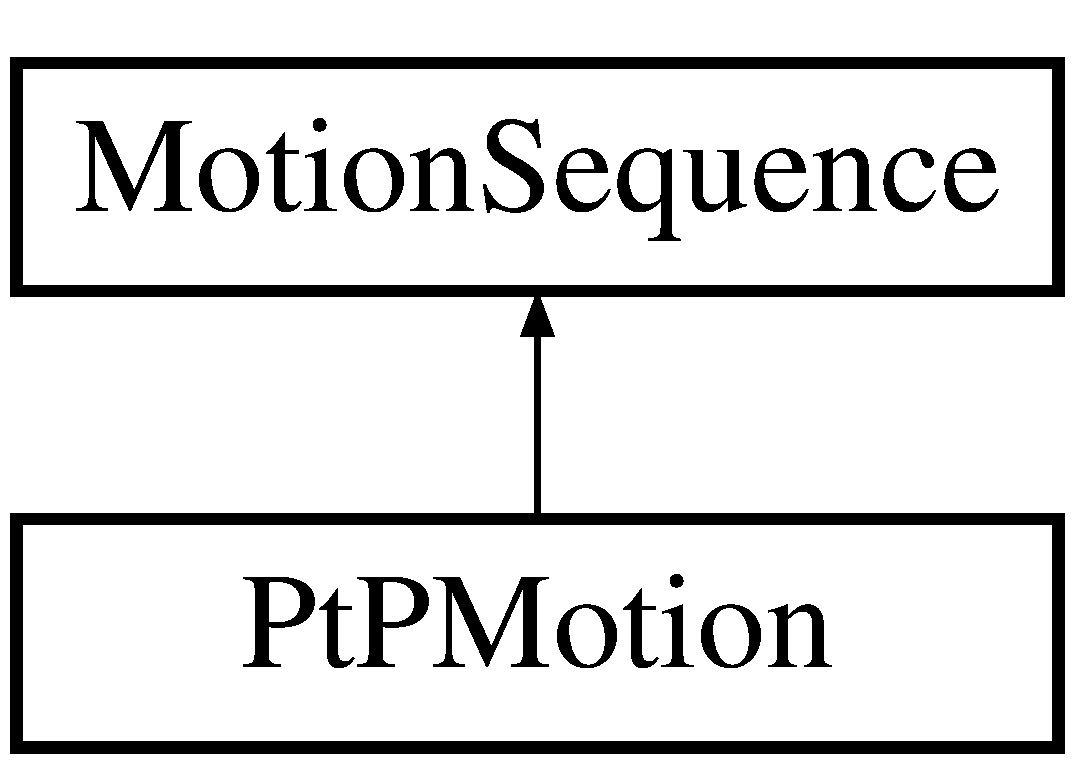
\includegraphics[height=2.000000cm]{class_pt_p_motion}
\end{center}
\end{figure}
\subsection*{Public Member Functions}
\begin{DoxyCompactItemize}
\item 
\mbox{\Hypertarget{class_pt_p_motion_acce1a2ec521ae2aa6c96fa42ddc5d954}\label{class_pt_p_motion_acce1a2ec521ae2aa6c96fa42ddc5d954}} 
{\bfseries Pt\+P\+Motion} (Speed\+Mode val\+Speed\+Mode, Position\+Mode val\+Position\+Mode)
\end{DoxyCompactItemize}


The documentation for this class was generated from the following files\+:\begin{DoxyCompactItemize}
\item 
Pt\+P\+Motion.\+h\item 
Pt\+P\+Motion.\+cpp\end{DoxyCompactItemize}

\hypertarget{class_robot_control}{}\section{Robot\+Control Class Reference}
\label{class_robot_control}\index{Robot\+Control@{Robot\+Control}}
\subsection*{Public Member Functions}
\begin{DoxyCompactItemize}
\item 
\mbox{\Hypertarget{class_robot_control_af8dcc887d6a52fe6b94523c8b9ecf746}\label{class_robot_control_af8dcc887d6a52fe6b94523c8b9ecf746}} 
{\bfseries run} ()
\item 
\mbox{\Hypertarget{class_robot_control_a530d619e20fa880ba539d270b508487e}\label{class_robot_control_a530d619e20fa880ba539d270b508487e}} 
{\bfseries test\+Functions} ()
\item 
\mbox{\Hypertarget{class_robot_control_aa8cc8dacbf9f4e6b232668105ab15a19}\label{class_robot_control_aa8cc8dacbf9f4e6b232668105ab15a19}} 
{\bfseries test\+Servo\+Adjustment} ()
\item 
\mbox{\Hypertarget{class_robot_control_a4adabcdcfaccaa079c4a540c53e4daaa}\label{class_robot_control_a4adabcdcfaccaa079c4a540c53e4daaa}} 
{\bfseries test\+Android\+Bluetooth} ()
\item 
\mbox{\Hypertarget{class_robot_control_ad1ce8b08753ec13739406daf49d2135d}\label{class_robot_control_ad1ce8b08753ec13739406daf49d2135d}} 
{\bfseries test\+Simple\+Bluetooth} ()
\item 
\mbox{\Hypertarget{class_robot_control_a66b5d4c35af5be7384bb45534007964e}\label{class_robot_control_a66b5d4c35af5be7384bb45534007964e}} 
{\bfseries test\+Inverse\+Kinematic} ()
\item 
\mbox{\Hypertarget{class_robot_control_a91851748b94bdc8680b146f9402bfde5}\label{class_robot_control_a91851748b94bdc8680b146f9402bfde5}} 
{\bfseries test\+\_\+interpolation\+Angle\+For\+Sync\+Lin\+Movement} ()
\item 
\mbox{\Hypertarget{class_robot_control_a0673868579c41fa105ab1e763521ba29}\label{class_robot_control_a0673868579c41fa105ab1e763521ba29}} 
{\bfseries test\+\_\+time\+Consumption\+Of\+One\+Step\+Calculations} ()
\item 
\mbox{\Hypertarget{class_robot_control_a2e2f908b8001a0dcc5702b16ccd8ef26}\label{class_robot_control_a2e2f908b8001a0dcc5702b16ccd8ef26}} 
{\bfseries test\+\_\+\+I\+CS} ()
\item 
\mbox{\Hypertarget{class_robot_control_acbeb418614406725e69cb441e7882b31}\label{class_robot_control_acbeb418614406725e69cb441e7882b31}} 
{\bfseries test\+\_\+step\+Machine} ()
\item 
\mbox{\Hypertarget{class_robot_control_a392598a8c4957b06394822f084ea098c}\label{class_robot_control_a392598a8c4957b06394822f084ea098c}} 
{\bfseries test\+\_\+all\+Legs\+Together} ()
\item 
\mbox{\Hypertarget{class_robot_control_a5bcaef8d9e58c70f582a2e9b2b42d807}\label{class_robot_control_a5bcaef8d9e58c70f582a2e9b2b42d807}} 
{\bfseries test\+\_\+leg1\+Correct\+Movement} ()
\end{DoxyCompactItemize}


The documentation for this class was generated from the following files\+:\begin{DoxyCompactItemize}
\item 
Robot\+Control.\+h\item 
Robot\+Control.\+cpp\end{DoxyCompactItemize}

\hypertarget{class_servo}{}\section{Servo Class Reference}
\label{class_servo}\index{Servo@{Servo}}
\subsection*{Public Member Functions}
\begin{DoxyCompactItemize}
\item 
\mbox{\Hypertarget{class_servo_affd2df4e8de8de0114398c04a4e6d6e0}\label{class_servo_affd2df4e8de8de0114398c04a4e6d6e0}} 
{\bfseries Servo} (A\+X12A \&m\+\_\+p\+Connected\+Bus, unsigned char ID)
\item 
\mbox{\Hypertarget{class_servo_aff9741ce884a22efcaa6476005db74d4}\label{class_servo_aff9741ce884a22efcaa6476005db74d4}} 
unsigned char {\bfseries set\+Max\+Angle} (float val)
\item 
\mbox{\Hypertarget{class_servo_a3cc0174ac451eea0391a27d40b15deda}\label{class_servo_a3cc0174ac451eea0391a27d40b15deda}} 
unsigned char {\bfseries set\+Min\+Angle} (float val)
\item 
\mbox{\Hypertarget{class_servo_ab0e99ff577c85efda55a4a44012e7e22}\label{class_servo_ab0e99ff577c85efda55a4a44012e7e22}} 
unsigned char {\bfseries set\+Servo\+Angle} (float angle\+Value)
\item 
\mbox{\Hypertarget{class_servo_a8ba146e7578f05ce76b13526eb9cf89c}\label{class_servo_a8ba146e7578f05ce76b13526eb9cf89c}} 
unsigned char {\bfseries set\+Servo\+Angle\+And\+Speed} (float angle\+Value, float speed)
\item 
\mbox{\Hypertarget{class_servo_a52a01b9ab1aef5a18944d4d96d151510}\label{class_servo_a52a01b9ab1aef5a18944d4d96d151510}} 
unsigned char {\bfseries set\+Servo\+Angle\+And\+Speed\+Reg} (float angle\+Value, float speed)
\item 
\mbox{\Hypertarget{class_servo_aa5cf66024865204126dff3270fa94a45}\label{class_servo_aa5cf66024865204126dff3270fa94a45}} 
int {\bfseries get\+Current\+Angle} ()
\item 
\mbox{\Hypertarget{class_servo_a0b23db9f7298f293b2a482af323754bd}\label{class_servo_a0b23db9f7298f293b2a482af323754bd}} 
int {\bfseries get\+Current\+Speed} ()
\end{DoxyCompactItemize}
\subsection*{Public Attributes}
\begin{DoxyCompactItemize}
\item 
\mbox{\Hypertarget{class_servo_a6bf385f763afedca0b3e62f2087e0dce}\label{class_servo_a6bf385f763afedca0b3e62f2087e0dce}} 
A\+X12A $\ast$ {\bfseries m\+\_\+p\+Connected\+Bus}
\item 
\mbox{\Hypertarget{class_servo_aa6997ed5b3ee0bc9920489f2a8e0bdb4}\label{class_servo_aa6997ed5b3ee0bc9920489f2a8e0bdb4}} 
unsigned char {\bfseries ID}
\item 
\mbox{\Hypertarget{class_servo_acd6a8ef2a2a182c2fb69365ab8a2749f}\label{class_servo_acd6a8ef2a2a182c2fb69365ab8a2749f}} 
float {\bfseries m\+\_\+max\+Angle}
\item 
\mbox{\Hypertarget{class_servo_a764996cbde84b094c960237194d46c36}\label{class_servo_a764996cbde84b094c960237194d46c36}} 
float {\bfseries m\+\_\+min\+Angle}
\item 
\mbox{\Hypertarget{class_servo_ae287d3e21ecc9f09552d58f1f07f16ab}\label{class_servo_ae287d3e21ecc9f09552d58f1f07f16ab}} 
float {\bfseries m\+\_\+max\+Speed}
\end{DoxyCompactItemize}


The documentation for this class was generated from the following files\+:\begin{DoxyCompactItemize}
\item 
Servo.\+h\item 
Servo.\+cpp\end{DoxyCompactItemize}

\chapter{File Documentation}
\hypertarget{_movement_controller_8cpp}{}\section{Movement\+Controller.\+cpp File Reference}
\label{_movement_controller_8cpp}\index{Movement\+Controller.\+cpp@{Movement\+Controller.\+cpp}}
{\ttfamily \#include \char`\"{}Movement\+Controller.\+h\char`\"{}}\newline
{\ttfamily \#include \char`\"{}A\+X12\+A.\+h\char`\"{}}\newline
{\ttfamily \#include $<$math.\+h$>$}\newline
\subsection*{Macros}
\begin{DoxyCompactItemize}
\item 
\mbox{\Hypertarget{_movement_controller_8cpp_a84982ac69f5ea07126a5ad08326242a5}\label{_movement_controller_8cpp_a84982ac69f5ea07126a5ad08326242a5}} 
\#define {\bfseries l01a}~119.\+845		/$\ast$mm$\ast$/
\item 
\mbox{\Hypertarget{_movement_controller_8cpp_aa53d4b178d5be08075374259f9c08a16}\label{_movement_controller_8cpp_aa53d4b178d5be08075374259f9c08a16}} 
\#define {\bfseries l01b}~47.\+75	 	/$\ast$mm$\ast$/
\item 
\mbox{\Hypertarget{_movement_controller_8cpp_a93b20dd0d13c8b3d12bb440daf01054f}\label{_movement_controller_8cpp_a93b20dd0d13c8b3d12bb440daf01054f}} 
\#define {\bfseries l12}~76.\+395      /$\ast$mm$\ast$/
\item 
\mbox{\Hypertarget{_movement_controller_8cpp_a7b8a07211c1a8b5b50581b687a47452e}\label{_movement_controller_8cpp_a7b8a07211c1a8b5b50581b687a47452e}} 
\#define {\bfseries l23}~204.\+33	    /$\ast$mm$\ast$/
\item 
\mbox{\Hypertarget{_movement_controller_8cpp_afb0a39e62ddb7c30992691af0a3a147b}\label{_movement_controller_8cpp_afb0a39e62ddb7c30992691af0a3a147b}} 
\#define {\bfseries l12quad}~pow(l12,2)
\item 
\mbox{\Hypertarget{_movement_controller_8cpp_a05fdc81c9f5d9804a7228a1d81fcc13c}\label{_movement_controller_8cpp_a05fdc81c9f5d9804a7228a1d81fcc13c}} 
\#define {\bfseries l23quad}~pow(l23,2)
\item 
\mbox{\Hypertarget{_movement_controller_8cpp_a61086ae7feef2874af228f8ce9ac4a46}\label{_movement_controller_8cpp_a61086ae7feef2874af228f8ce9ac4a46}} 
\#define {\bfseries bmax}~4956.\+084 /$\ast$deg/sec$^\wedge$2$\ast$/
\item 
\mbox{\Hypertarget{_movement_controller_8cpp_a1c8f52db51d2e3c5f5e07956d1705123}\label{_movement_controller_8cpp_a1c8f52db51d2e3c5f5e07956d1705123}} 
\#define {\bfseries vmax}~684.\+0/2 /$\ast$deg/sec$^\wedge$2$\ast$/
\item 
\mbox{\Hypertarget{_movement_controller_8cpp_abf172ffa86dcc11c95aeeebee7031830}\label{_movement_controller_8cpp_abf172ffa86dcc11c95aeeebee7031830}} 
\#define {\bfseries c\+\_\+k}~sqrt(pow(l01a,2)+pow(l01b,2))
\item 
\mbox{\Hypertarget{_movement_controller_8cpp_acbf88d402c6bef14d80b3109e42b237a}\label{_movement_controller_8cpp_acbf88d402c6bef14d80b3109e42b237a}} 
\#define {\bfseries c\+\_\+phi}~M\+\_\+\+PI / 6.\+0
\item 
\mbox{\Hypertarget{_movement_controller_8cpp_aa57579f9bf10717f8ee88c88eea352ce}\label{_movement_controller_8cpp_aa57579f9bf10717f8ee88c88eea352ce}} 
\#define {\bfseries c\+\_\+kquad}~pow(c\+\_\+k,2)
\item 
\mbox{\Hypertarget{_movement_controller_8cpp_a15fd2e784e91357a12047d9e7dcabb5b}\label{_movement_controller_8cpp_a15fd2e784e91357a12047d9e7dcabb5b}} 
\#define {\bfseries c\+\_\+gamma}~atan(l01b/l01a)
\item 
\mbox{\Hypertarget{_movement_controller_8cpp_afa7039aefb12b7d57f270230b835dcda}\label{_movement_controller_8cpp_afa7039aefb12b7d57f270230b835dcda}} 
\#define {\bfseries c\+\_\+delta}~atan(l01a/l01b)
\item 
\mbox{\Hypertarget{_movement_controller_8cpp_acf490a3bcf76b324e5b280d3740d620e}\label{_movement_controller_8cpp_acf490a3bcf76b324e5b280d3740d620e}} 
\#define {\bfseries T\+\_\+\+I\+PO}~0.\+01f
\end{DoxyCompactItemize}
\begin{Indent}\textbf{ constant leg parameters}\par
{\em vector parts that starts from the origin of the world coordinate system to an origin of a leg coordinate system. Can be used for every leg, because the robot is symmetrical with respect to the x-\/axes A\+ND y-\/axes. Only the sign of those variables varies. (see documentation for further definition) }\begin{DoxyCompactItemize}
\item 
\mbox{\Hypertarget{_movement_controller_8cpp_a8f2d615cb39c3959c71f42b925f3c1e5}\label{_movement_controller_8cpp_a8f2d615cb39c3959c71f42b925f3c1e5}} 
\#define {\bfseries pwkx}~116.\+41
\item 
\mbox{\Hypertarget{_movement_controller_8cpp_aa9245231c8e4d3a2e20486d06b9023fb}\label{_movement_controller_8cpp_aa9245231c8e4d3a2e20486d06b9023fb}} 
\#define {\bfseries pwky}~79.\+379
\item 
\mbox{\Hypertarget{_movement_controller_8cpp_a2b1ec9f4b5ef449695b0ee74d5d38ebc}\label{_movement_controller_8cpp_a2b1ec9f4b5ef449695b0ee74d5d38ebc}} 
\#define {\bfseries pwkz}~666 /$\ast$T\+O\+D\+O\+: Unclear which parameter goes here!!!$\ast$/
\item 
\mbox{\Hypertarget{_movement_controller_8cpp_a746b50ea4e3c69607304a354fae0e519}\label{_movement_controller_8cpp_a746b50ea4e3c69607304a354fae0e519}} 
\#define {\bfseries pwk\+Angle}~(30.\+0/180.\+0)$\ast$M\+\_\+\+PI
\end{DoxyCompactItemize}
\end{Indent}

\hypertarget{_movement_controller_8h}{}\section{Movement\+Controller.\+h File Reference}
\label{_movement_controller_8h}\index{Movement\+Controller.\+h@{Movement\+Controller.\+h}}
{\ttfamily \#include \char`\"{}Leg.\+h\char`\"{}}\newline
{\ttfamily \#include \char`\"{}Arduino.\+h\char`\"{}}\newline
{\ttfamily \#include \char`\"{}A\+X12\+A.\+h\char`\"{}}\newline
\subsection*{Classes}
\begin{DoxyCompactItemize}
\item 
class \mbox{\hyperlink{class_movement_controller}{Movement\+Controller}}
\end{DoxyCompactItemize}
\subsection*{Macros}
\begin{Indent}\textbf{ U\+A\+RT settings}\par
\begin{DoxyCompactItemize}
\item 
\mbox{\Hypertarget{_movement_controller_8h_a61b7473eb445c16d3b943f864fa94af1}\label{_movement_controller_8h_a61b7473eb445c16d3b943f864fa94af1}} 
\#define {\bfseries Direction\+Pin\+For\+Bus1}~(10u)
\item 
\mbox{\Hypertarget{_movement_controller_8h_a844b7e04baaa249e0ebe537a2b666f15}\label{_movement_controller_8h_a844b7e04baaa249e0ebe537a2b666f15}} 
\#define {\bfseries Baud\+Rate}~(1000000ul)
\item 
\mbox{\Hypertarget{_movement_controller_8h_a404421a44414b42adb50e85fc34b297c}\label{_movement_controller_8h_a404421a44414b42adb50e85fc34b297c}} 
\#define {\bfseries Servo\+Serial\+For\+Bus1}~(Serial1)
\item 
\mbox{\Hypertarget{_movement_controller_8h_afb79d569cd0fbe61692492dbe293f006}\label{_movement_controller_8h_afb79d569cd0fbe61692492dbe293f006}} 
\#define {\bfseries Direction\+Pin\+For\+Bus2}~(10u)
\item 
\mbox{\Hypertarget{_movement_controller_8h_a844b7e04baaa249e0ebe537a2b666f15}\label{_movement_controller_8h_a844b7e04baaa249e0ebe537a2b666f15}} 
\#define {\bfseries Baud\+Rate}~(1000000ul)
\item 
\mbox{\Hypertarget{_movement_controller_8h_ad0b03cb0f4ff5c4cd2be1cff2ec7f1f6}\label{_movement_controller_8h_ad0b03cb0f4ff5c4cd2be1cff2ec7f1f6}} 
\#define {\bfseries Servo\+Serial\+For\+Bus2}~(Serial2)
\item 
\mbox{\Hypertarget{_movement_controller_8h_a21698bdf2eae333643ab8558da0e35cd}\label{_movement_controller_8h_a21698bdf2eae333643ab8558da0e35cd}} 
\#define {\bfseries Direction\+Pin\+For\+Bus3}~(10u)
\item 
\mbox{\Hypertarget{_movement_controller_8h_a844b7e04baaa249e0ebe537a2b666f15}\label{_movement_controller_8h_a844b7e04baaa249e0ebe537a2b666f15}} 
\#define {\bfseries Baud\+Rate}~(1000000ul)
\item 
\mbox{\Hypertarget{_movement_controller_8h_a54c9b38f5ac696572b447121d688e508}\label{_movement_controller_8h_a54c9b38f5ac696572b447121d688e508}} 
\#define {\bfseries Servo\+Serial\+For\+Bus3}~(Serial3)
\end{DoxyCompactItemize}
\end{Indent}
\begin{Indent}\textbf{ Servo ID\textquotesingle{}s}\par
{\em Predefined ID\textquotesingle{}s, that the servos are set to. }\begin{DoxyCompactItemize}
\item 
\mbox{\Hypertarget{_movement_controller_8h_a7af80c88c3c1f27e87cc4238bdf688e4}\label{_movement_controller_8h_a7af80c88c3c1f27e87cc4238bdf688e4}} 
\#define {\bfseries I\+D\+\_\+leg1\+\_\+lower\+Leg\+Servo}~3
\item 
\mbox{\Hypertarget{_movement_controller_8h_aeaa5c59e9d0ba33276af592b904e8e25}\label{_movement_controller_8h_aeaa5c59e9d0ba33276af592b904e8e25}} 
\#define {\bfseries I\+D\+\_\+leg1\+\_\+middle\+Leg\+Servo}~2
\item 
\mbox{\Hypertarget{_movement_controller_8h_afc4c31ff90919906cfa92b709dcae991}\label{_movement_controller_8h_afc4c31ff90919906cfa92b709dcae991}} 
\#define {\bfseries I\+D\+\_\+leg1\+\_\+body\+Servo}~1
\item 
\mbox{\Hypertarget{_movement_controller_8h_a30c224a3df46b1f0da71bbdee1e12116}\label{_movement_controller_8h_a30c224a3df46b1f0da71bbdee1e12116}} 
\#define {\bfseries I\+D\+\_\+leg2\+\_\+lower\+Leg\+Servo}~4
\item 
\mbox{\Hypertarget{_movement_controller_8h_a4e3f4a532c8d8505dba29d09b51021cd}\label{_movement_controller_8h_a4e3f4a532c8d8505dba29d09b51021cd}} 
\#define {\bfseries I\+D\+\_\+leg2\+\_\+middle\+Leg\+Servo}~5
\item 
\mbox{\Hypertarget{_movement_controller_8h_aabc6c88cc8c4e1495a73b1da61516126}\label{_movement_controller_8h_aabc6c88cc8c4e1495a73b1da61516126}} 
\#define {\bfseries I\+D\+\_\+leg2\+\_\+body\+Servo}~6
\item 
\mbox{\Hypertarget{_movement_controller_8h_a328af6085722e60023adc1bc0825fa5a}\label{_movement_controller_8h_a328af6085722e60023adc1bc0825fa5a}} 
\#define {\bfseries I\+D\+\_\+leg3\+\_\+lower\+Leg\+Servo}~7
\item 
\mbox{\Hypertarget{_movement_controller_8h_a81bd7025dd0eb8c216b12af02b850711}\label{_movement_controller_8h_a81bd7025dd0eb8c216b12af02b850711}} 
\#define {\bfseries I\+D\+\_\+leg3\+\_\+middle\+Leg\+Servo}~8
\item 
\mbox{\Hypertarget{_movement_controller_8h_a999c1a48c57f670be23bc05e2aeb2d94}\label{_movement_controller_8h_a999c1a48c57f670be23bc05e2aeb2d94}} 
\#define {\bfseries I\+D\+\_\+leg3\+\_\+body\+Servo}~9
\item 
\mbox{\Hypertarget{_movement_controller_8h_a9fcf88e44a37e369d5d5c7abc552c6c3}\label{_movement_controller_8h_a9fcf88e44a37e369d5d5c7abc552c6c3}} 
\#define {\bfseries I\+D\+\_\+leg4\+\_\+lower\+Leg\+Servo}~10
\item 
\mbox{\Hypertarget{_movement_controller_8h_a21f8fa56cd2720cf7bba3c7202a49b88}\label{_movement_controller_8h_a21f8fa56cd2720cf7bba3c7202a49b88}} 
\#define {\bfseries I\+D\+\_\+leg4\+\_\+middle\+Leg\+Servo}~11
\item 
\mbox{\Hypertarget{_movement_controller_8h_a48f61fd0a39ebd13b4a8897f1fddffbb}\label{_movement_controller_8h_a48f61fd0a39ebd13b4a8897f1fddffbb}} 
\#define {\bfseries I\+D\+\_\+leg4\+\_\+body\+Servo}~12
\item 
\mbox{\Hypertarget{_movement_controller_8h_a15ecc05e2e2712d8446dcc2383e80b99}\label{_movement_controller_8h_a15ecc05e2e2712d8446dcc2383e80b99}} 
\#define {\bfseries I\+D\+\_\+leg5\+\_\+lower\+Leg\+Servo}~13
\item 
\mbox{\Hypertarget{_movement_controller_8h_a87854198ac831c950ea4b4ed2640e18d}\label{_movement_controller_8h_a87854198ac831c950ea4b4ed2640e18d}} 
\#define {\bfseries I\+D\+\_\+leg5\+\_\+middle\+Leg\+Servo}~14
\item 
\mbox{\Hypertarget{_movement_controller_8h_a21fa5d9acea0a9959e0cbd4c3ab84e3e}\label{_movement_controller_8h_a21fa5d9acea0a9959e0cbd4c3ab84e3e}} 
\#define {\bfseries I\+D\+\_\+leg5\+\_\+body\+Servo}~15
\item 
\mbox{\Hypertarget{_movement_controller_8h_a804c83929826c18ab176b0ffab1d70d9}\label{_movement_controller_8h_a804c83929826c18ab176b0ffab1d70d9}} 
\#define {\bfseries I\+D\+\_\+leg6\+\_\+lower\+Leg\+Servo}~16
\item 
\mbox{\Hypertarget{_movement_controller_8h_a73676e6c7cc00e219b3942d6be8db4d3}\label{_movement_controller_8h_a73676e6c7cc00e219b3942d6be8db4d3}} 
\#define {\bfseries I\+D\+\_\+leg6\+\_\+middle\+Leg\+Servo}~17
\item 
\mbox{\Hypertarget{_movement_controller_8h_a1b6a807a20437121d6ea7ab419192d8f}\label{_movement_controller_8h_a1b6a807a20437121d6ea7ab419192d8f}} 
\#define {\bfseries I\+D\+\_\+leg6\+\_\+body\+Servo}~18
\end{DoxyCompactItemize}
\end{Indent}

%--- End generated contents ---

% Index
\backmatter
\newpage
\phantomsection
\clearemptydoublepage
\addcontentsline{toc}{chapter}{Index}
\printindex

\end{document}
